\chapter{Validacion}
\label{sec:validacion}



% Explicando el propósito y la estrategia general de la validación
El objetivo de esta fase es demostrar, mediante evidencias reproducibles, que el prototipo desarrollado cumple con los requisitos funcionales \textbf{RF-01} a \textbf{RF-06} y los no funcionales \textbf{RNF-01} a \textbf{RNF-03}, definidos en el Capítulo 3, así como con las reglas establecidas en el \textit{SRTP Scheme Rulebook v4.0}. Para lograr esto, se diseñó una estrategia de validación escalonada que combina pruebas manuales exploratorias, una batería de pruebas automatizadas ejecutadas con Postman, y la inspección de \textit{logs} hashados que garantizan la trazabilidad del ciclo de vida de cada solicitud RTP. En esta sección se describe en detalle la metodología empleada, el entorno de pruebas, los escenarios cubiertos y los resultados obtenidos.

% Detallando el entorno de pruebas
\section{Entorno de pruebas}

El entorno de pruebas se configuró utilizando las siguientes herramientas y configuraciones:

\begin{itemize}
  \item \textbf{Herramientas}: Se utilizó Postman v10 para la construcción y envío de peticiones HTTP, SQLite 3 como base de datos, y la utilidad integrada de \textit{Flask-SocketIO} para la inspección de eventos en tiempo real.
  
  \item \textbf{Variable de entorno \texttt{baseURL}}: Antes de crear la colección de pruebas, se definió la variable \texttt{baseURL} con la URL base del servidor (véase Fig.~\ref{fig:baseURL}). Esto permite evitar la repetición de la URL completa en cada petición y facilita el cambio entre entornos (por ejemplo, de desarrollo a integración continua) con una sola modificación.
  
  \item \textbf{Datos semilla}: Al iniciar la aplicación, el archivo \texttt{app.py} crea automáticamente cuatro actores predefinidos. Estos actores cuentan con saldos, relaciones y roles preestablecidos, lo que permite ejecutar los flujos de prueba sin necesidad de pasos adicionales de alta de usuarios.
\end{itemize}

% Describiendo la metodología de pruebas
\section{Metodología}

La metodología de validación se estructuró en tres etapas principales:

\begin{enumerate}
  \item \textbf{Pruebas exploratorias}: En las primeras iteraciones del desarrollo, cuando el prototipo solo exponía la API REST, se empleó un ciclo manual de \textit{definir petición → enviar → analizar respuesta → refactorizar código} para depurar la lógica de negocio. Durante esta etapa, se mantuvieron \textit{endpoints} internos, como \texttt{/actor} (véase Fig.~\ref{fig:crearActor}), que, aunque ya no están expuestos en la interfaz web, siguen disponibles para escenarios de administración.
  
  \item \textbf{Colección Postman}: Una vez estabilizada la API, se preparó la colección \textit{MiAPITFG} (véase Fig.~\ref{fig:MiAPITFG}), que orquesta las llamadas clave del flujo RTP y verifica los códigos de estado HTTP, los cuerpos de respuesta JSON y la correcta transición de estados de la entidad \texttt{RTP}. Cada vez que se modifica el código, esta colección se ejecuta localmente.
  
  \item \textbf{Cobertura y trazabilidad}: Todas las pruebas están enlazadas con los requisitos y la función \texttt{cambiar\_estado\_rtp} registra un hash de los datos críticos cada vez que se produce un cambio de estado en una solicitud RTP, garantizando así la integridad y trazabilidad de los resultados de las pruebas.
\end{enumerate}

% Presentando el flujo nominal (happy path)
\section{Flujo \textit{happy path}}

El flujo nominal, también conocido como \textit{happy path}, fue validado mediante la colección Postman, siguiendo los pasos descritos a continuación. Las capturas asociadas a cada paso se enumeran entre paréntesis.

\begin{enumerate}
  \item \textbf{Creación del RTP} (\texttt{/rtp}, Figs.~\ref{fig:crearRTP}–\ref{fig:crearRTPResponse}): El beneficiario envía una solicitud de cobro a un pagador identificado por su IBAN.
  
  \item \textbf{Validación y enrutado en el PSP del Beneficiario} (Figs.~\ref{fig:validarBenef}–\ref{fig:enrutarBenefResponse}): Se verifica la sintaxis de la solicitud (IBAN válido, importe positivo, etc.) y, si todo es correcto, se enruta la solicitud al PSP del pagador.
  
  \item \textbf{Validación en el PSP del Pagador} (Figs.~\ref{fig:validarPayer}–\ref{fig:validarPayerResponse}): El PSP del pagador comprueba el saldo disponible y aplica reglas simplificadas de KYC/AML.
  
  \item \textbf{Decisión del Pagador} (Figs.~\ref{fig:decision}–\ref{fig:decisionResponse}): El pagador acepta o rechaza la solicitud. La decisión se propaga en menos de 10 segundos mediante WebSocket, cumpliendo con el requisito funcional \textbf{RF-05}.
\end{enumerate}

En cada una de estas fases, se comprobaron los siguientes aspectos:

\begin{itemize}
  \item El código de estado HTTP es el adecuado (por ejemplo, 201 para creación, 200 para éxito, 400 para error).
  \item La consistencia del estado de la solicitud RTP en la base de datos y la emisión correcta del evento \texttt{rtp\_<estado>} en la sala correspondiente de WebSocket.
\end{itemize}

% Analizando los escenarios de error
\section{Escenarios de error}

Para verificar la resiliencia del sistema frente a situaciones adversas, se diseñaron y probaron tres escenarios de error comunes, todos ellos incorporados a la colección Postman para garantizar la regresión continua:

\begin{description}
  \item[IBAN inválido o no registrado]: La función \texttt{validar\_iban()} rechaza la solicitud con un código de estado \texttt{400 Bad Request}. Este caso se muestra en la captura Fig.~\ref{fig:error1}.
  
  \item[Saldo insuficiente]: El PSP del pagador detecta que el saldo es insuficiente y emite un \textbf{rechazo}. La colección confirma que el estado final de la solicitud RTP es \texttt{rejected}. Véase Figs.~\ref{fig:error2_1}–\ref{fig:error2_2}.
  
  \item[Actores inexistentes]: Si alguno de los actores requeridos no está presente en la base de datos, el servicio responde con \texttt{404 Not Found} y el flujo se detiene inmediatamente (Fig.~\ref{fig:error3}).
\end{description}

% Resumiendo las conclusiones de la validación
\section{Conclusiones}

La estrategia de validación adoptada ha demostrado que:

\begin{itemize}
  \item Los tres escenarios de error confirman la robustez del sistema frente a datos maliciosos o inconsistentes, alineándose con el requisito no funcional \textbf{RNF-02}.
  \item La integración continua impide que nuevas funcionalidades degraden la experiencia del usuario o comprometan la seguridad del sistema.
\end{itemize}

En consecuencia, el prototipo satisface las metas de validación establecidas al inicio del proyecto y proporciona una base sólida para futuras extensiones, como la integración con bancos reales o la realización de pruebas de carga, tal como se propone en el capítulo \ref{sec:Potencial}.



\begin{figure}[H]
  \centering
  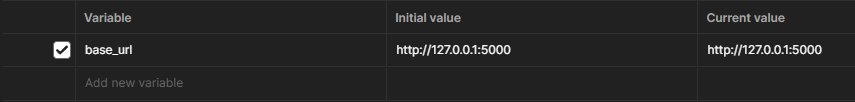
\includegraphics[width=0.8\textwidth]{Imagenes/baseURL.png}
  \caption{Variable \texttt{baseURL} en Postman}
  \label{fig:baseURL}
\end{figure}


\begin{figure}[H]
  \centering
  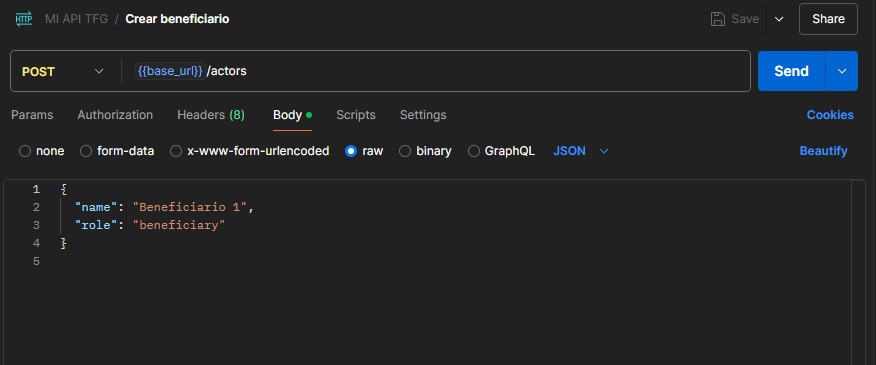
\includegraphics[width=0.8\textwidth]{Imagenes/crearActor.png}
  \caption{crearActor}
  \label{fig:crearActor}
\end{figure}

\begin{figure}[H]
  \centering
  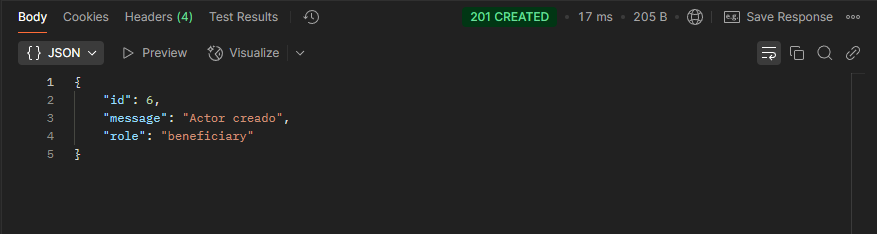
\includegraphics[width=0.8\textwidth]{Imagenes/crearActorResponse.png}
  \caption{crearActorResponse}
  \label{fig:crearActorResponse}
\end{figure}


\begin{figure}[H]
  \centering
  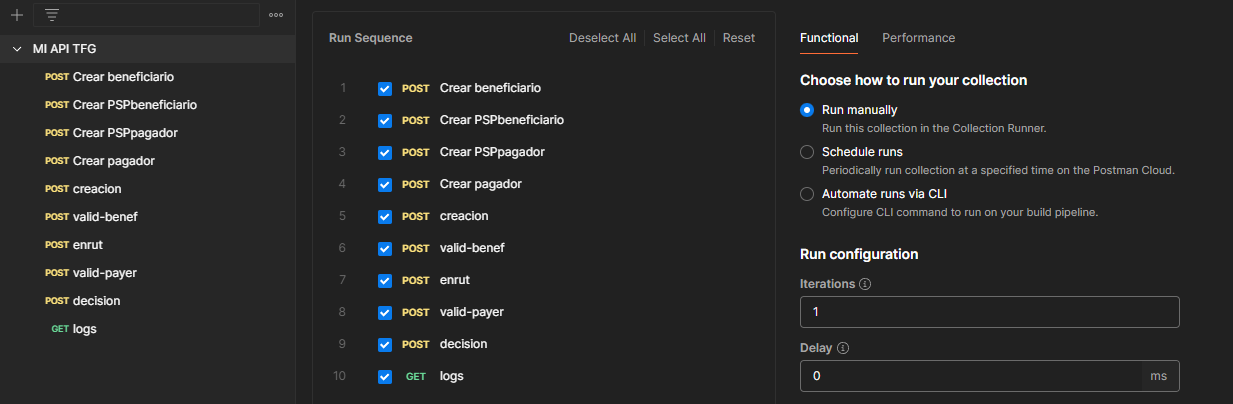
\includegraphics[width=0.8\textwidth]{Imagenes/MiAPITFG.png}
  \caption{MiAPITFG}
  \label{fig:MiAPITFG}
\end{figure}

\begin{figure}[H]
  \centering
  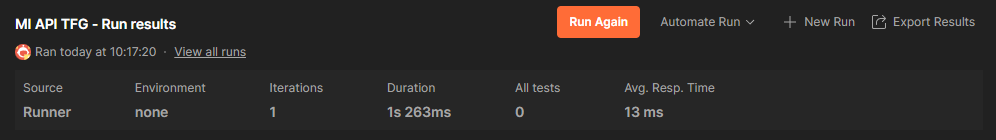
\includegraphics[width=0.8\textwidth]{Imagenes/RunResults.png}
  \caption{RunResults}
  \label{fig:RunResults}
\end{figure}



    \begin{figure}[H]
    \centering
    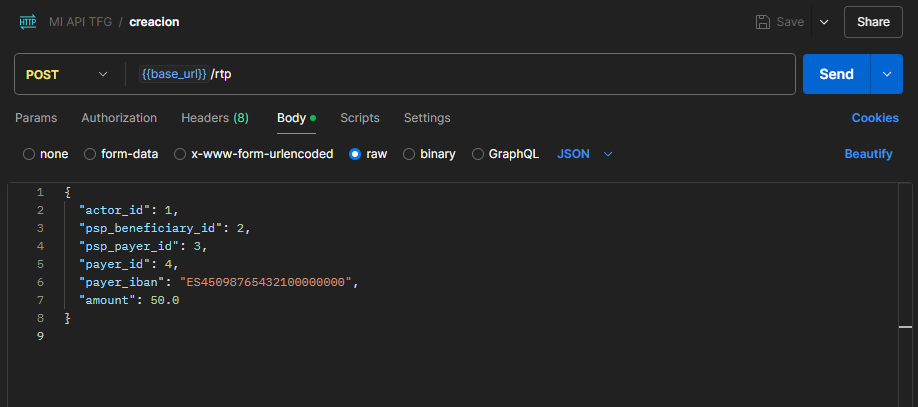
\includegraphics[width=0.8\textwidth]{Imagenes/crearRTP.png}
    \caption{crearRTP}
    \label{fig:crearRTP}
    \end{figure}

    \begin{figure}[H]
    \centering
    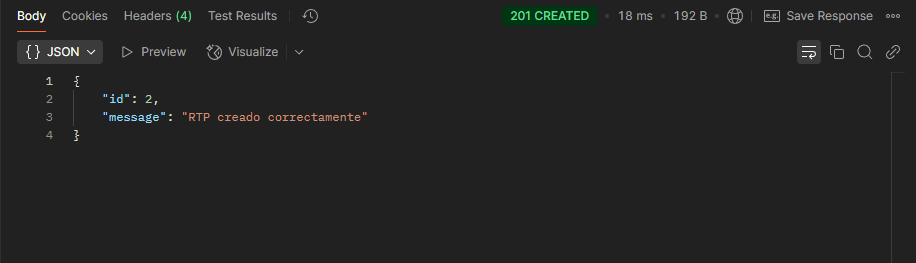
\includegraphics[width=0.8\textwidth]{Imagenes/crearRTPResponse.png}
    \caption{crearRTPResponse}
    \label{fig:crearRTPResponse}
    \end{figure}

    \begin{figure}[H]
    \centering
    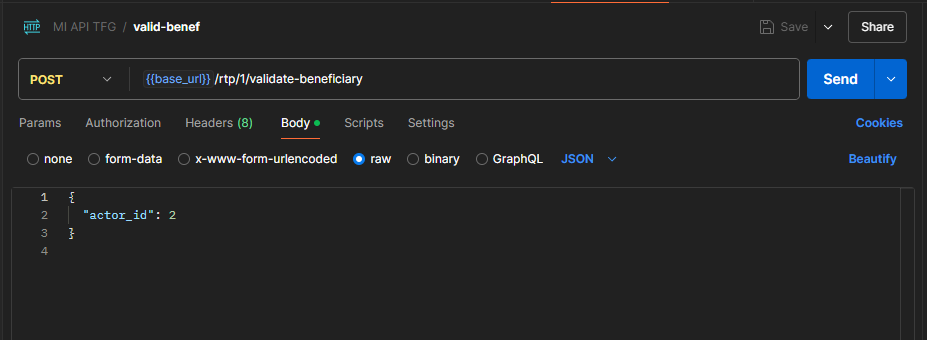
\includegraphics[width=0.8\textwidth]{Imagenes/validarBenef.png}
    \caption{validarBenef}
    \label{fig:validarBenef}
    \end{figure}

    \begin{figure}[H]
    \centering
    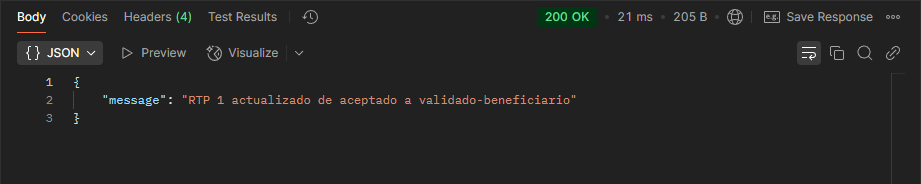
\includegraphics[width=0.8\textwidth]{Imagenes/validarBenefResponse.png}
    \caption{validarBenefResponse}
    \label{fig:validarBenefResponse}
    \end{figure}

    \begin{figure}[H]
    \centering
    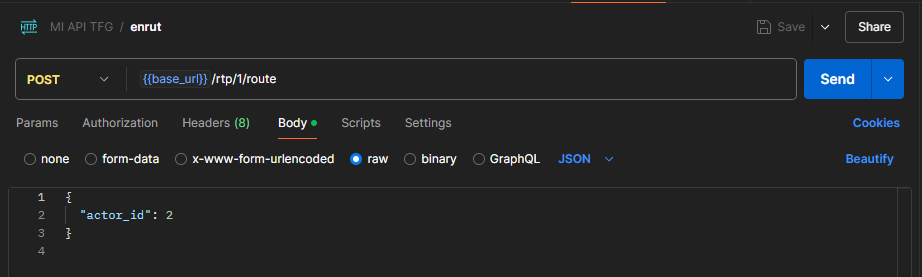
\includegraphics[width=0.8\textwidth]{Imagenes/enrutarBenef.png}
    \caption{enrutarBenef}
    \label{fig:enrutarBenef}
    \end{figure}


    \begin{figure}[H]
    \centering
    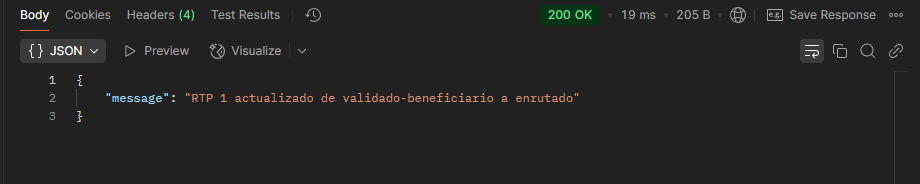
\includegraphics[width=0.8\textwidth]{Imagenes/enrutarBenefResponse.png}
    \caption{enrutarBenefResponse}
    \label{fig:enrutarBenefResponse}
    \end{figure}



    \begin{figure}[H]
    \centering
    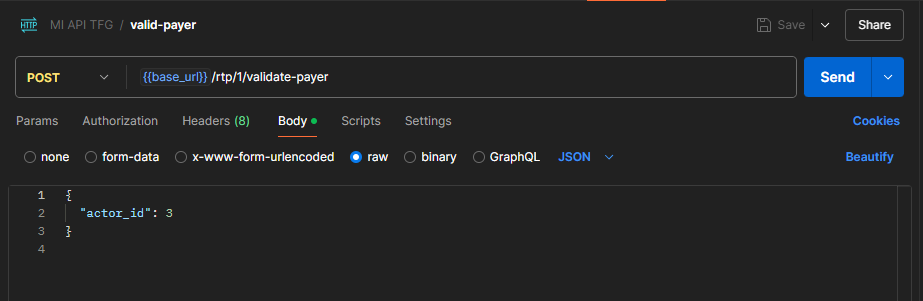
\includegraphics[width=0.8\textwidth]{Imagenes/validarPayer.png}
    \caption{validarPayer}
    \label{fig:validarPayer}
    \end{figure}

    \begin{figure}[H]
    \centering
    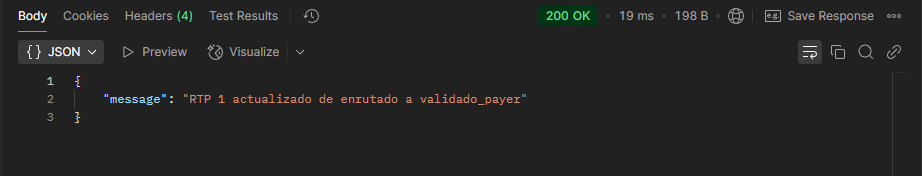
\includegraphics[width=0.8\textwidth]{Imagenes/validarPayerResponse.png}
    \caption{validarPayerResponse}
    \label{fig:validarPayerResponse}
    \end{figure}



    \begin{figure}[H]
    \centering
    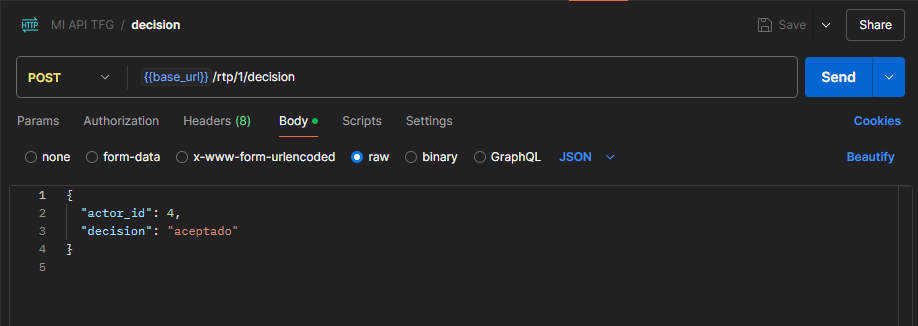
\includegraphics[width=0.8\textwidth]{Imagenes/decision.png}
    \caption{decision}
    \label{fig:decision}
    \end{figure}

    \begin{figure}[H]
    \centering
    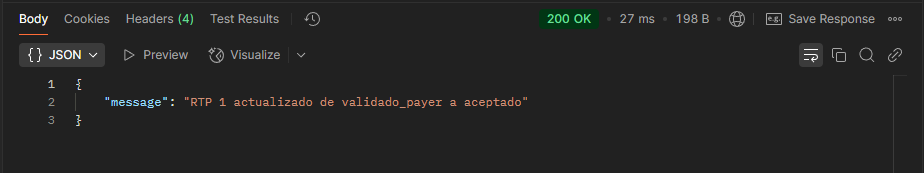
\includegraphics[width=0.8\textwidth]{Imagenes/decisionResponse.png}
    \caption{decisionResponse}
    \label{fig:decisionResponse}
    \end{figure}



    \begin{figure}[H]
    \centering
    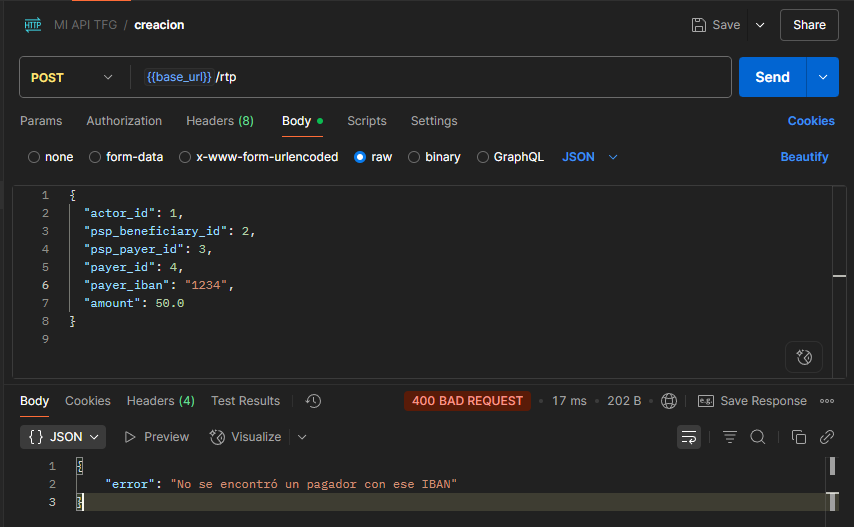
\includegraphics[width=0.8\textwidth]{Imagenes/error1.png}
    \caption{error1}
    \label{fig:error1}
    \end{figure}

    \begin{figure}[H]
    \centering
    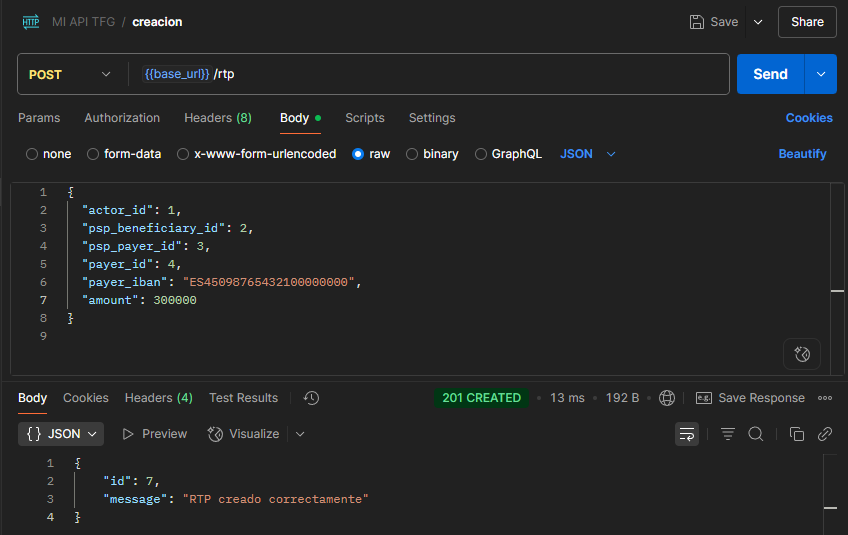
\includegraphics[width=0.8\textwidth]{Imagenes/error2_1.png}
    \caption{error2\_1}
    \label{fig:error2_1}
    \end{figure}

    \begin{figure}[H]
    \centering
    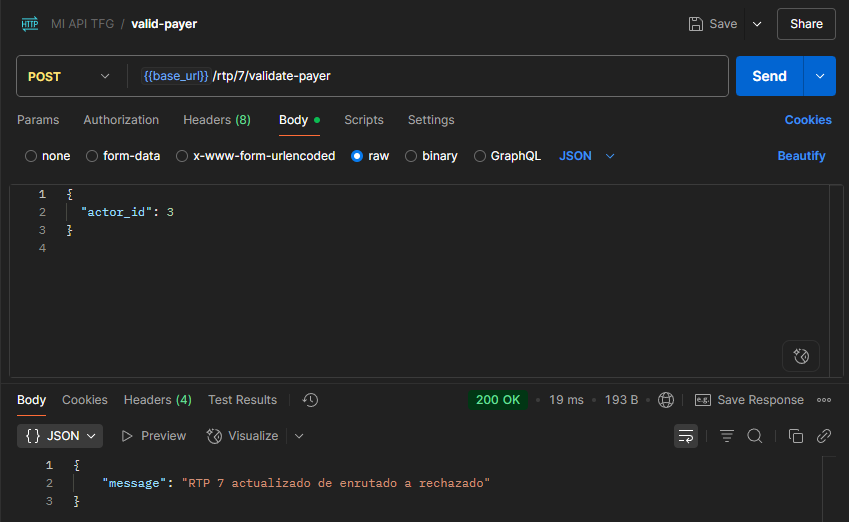
\includegraphics[width=0.8\textwidth]{Imagenes/error2_2.png}
    \caption{error2\_2}
    \label{fig:error2_2}
    \end{figure}


    \begin{figure}[H]
    \centering
    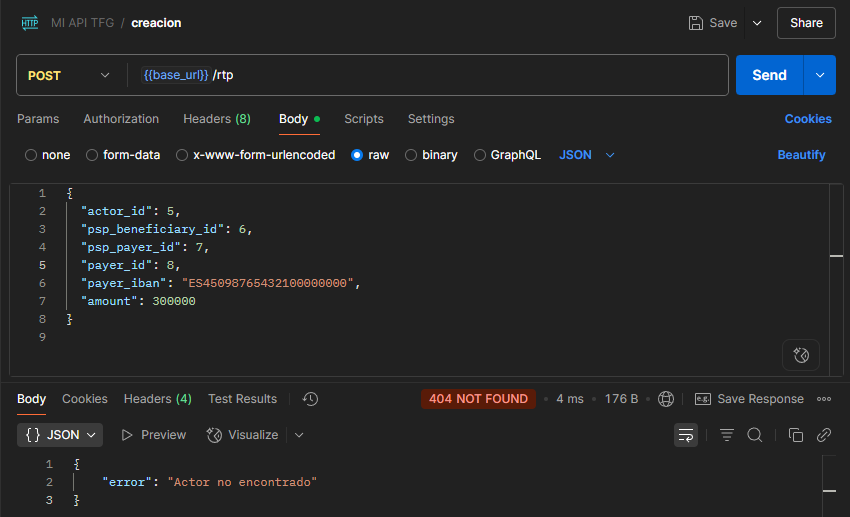
\includegraphics[width=0.8\textwidth]{Imagenes/error3.png}
    \caption{error3}
    \label{fig:error3}
    \end{figure}
